\documentclass[a4paper,12pt]{article}
\usepackage[utf8]{inputenc}
\usepackage[T2A]{fontenc}
\usepackage[russian]{babel}
\usepackage{amsthm}
\usepackage{amsmath}
\usepackage{amssymb}
\usepackage{tikz}
\usepackage{textcomp}
\usepackage{marvosym}
\usepackage{esint}
\usepackage{graphicx}
\usepackage{float}
\usepackage{wrapfig}
\usepackage{pgfplots}
\usepackage{caption}
\usepackage{array}
\usepackage{booktabs}
\usepackage{geometry}

\geometry{a4paper,
    left=20mm,
    right=20mm,
    top=20mm,
    bottom=20mm}

\pgfplotsset{compat=1.16}
\graphicspath{ {./images/} }

\setlength{\topmargin}{-0.5in}
\setlength{\textheight}{9.1in}
\setlength{\oddsidemargin}{-0.4in}
\setlength{\evensidemargin}{-0.4in}
\setlength{\textwidth}{7in}
\setlength{\parindent}{0ex}
\setlength{\parskip}{1ex}

\newcommand{\ndiv}{\hspace{-4pt}\not|\hspace{2pt}}

\title{Лабораторная работа № 3.6.1\\Спектральный анализ электрических сигналов}
\author{Меркулов Кирилл}
\date{\today}

\begin{document}

\maketitle
\newpage

\section*{Введение}

\textbf{В работе используются:} генератор сигналов произвольной формы, цифровой осциллограф с функцией быстрого преобразования Фурье или цифровой USB-осциллограф, подключённый к персональному компьютеру.

\textbf{Цель работы:} изучить спектры сигналов различной формы и влияние параметров сигнала на вид соответствующих спектров; проверить справедливость соотношений неопределённостей; познакомиться с работой спектральных фильтров на примере RC-цепочки.

\subsection*{Ряд Фурье и спектральный анализ}

Согласно теореме Фурье, любая периодическая функция может быть представлена в виде ряда (конечного или бесконечного) гармонических функций с кратными частотами — ряда Фурье. Одно из представлений ряда Фурье для функции с периодом $T$ имеет вид
\[
f(t) = \frac{A_0}{2} + \sum_{n=1}^{\infty}A_n \cdot \cos(2 \cdot \pi \cdot \nu_n \cdot t) + B_n \cdot \sin(2 \cdot \pi \cdot \nu_n \cdot t),
\]
где $\nu_n = n \cdot \nu_0$, $\nu_0 = \frac{1}{T}$, $n = 1,2, \ldots$ — частоты фурье-гармоник, $A_n$ и $B_n$ — коэффициенты разложения в ряд Фурье. Коэффициенты находятся как
\[
A_n = \frac{2}{T} \cdot \int_0^T f(t) \cdot \cos(2 \cdot \pi \cdot \nu_n \cdot t) dt,
\]
\[
B_n = \frac{2}{T} \cdot \int_0^T f(t) \cdot \sin(2 \cdot \pi \cdot \nu_n \cdot t) dt.
\]

На практике зачастую удобнее использовать эквивалентную форму записи ряда Фурье в «представлении амплитуд и фаз»:
\[
f(t) = \frac{a_0}{2} + \sum_{n=1}^{\infty} a_n \cdot \cos(2 \cdot \pi \cdot \nu_n \cdot t + \varphi_n),
\]
где по известной тригонометрической формуле амплитуда гармоники равна $a_n = \sqrt{A_n^2 + B_n^2}$, а фаза определяется соотношением $\tan(\varphi_n) = \frac{B_n}{A_n}$.

Отметим, что если функция f чётная, то $B_n \equiv 0$ ($\varphi_n \equiv 0$, разложение по косинусам), а если нечётная, то $A_n \equiv 0$ ($\varphi \equiv \frac{\pi}{2}$, разложение по синусам).

Совокупность всех частот $\nu_n$ и соответствующих им амплитуд $a_n$ (а также фаз $\varphi_n$) часто называют спектром функции $f(t)$. Если речь идёт об изменяющемся во времени напряжении, то говорят о спектре электрического сигнала.

Спектральный анализ электрических сигналов играет важную роль в технике. Особенно важен он для линейных систем, подчиняющихся принципу суперпозиции. Если известно, как некоторая система реагирует на гармонический сигнал, с помощью разложения Фурье можно определить, как система будет реагировать на произвольную функцию $f(t)$.

Заметим, что спектр периодической функции дискретен (число гармоник счётно). Если функция не периодическая (но ограниченная во времени, например, отдельный «импульс»), её можно представить как предел периодической функции с очень большим периодом $T \rightarrow \infty$. Тогда частотное расстояние между соседними гармониками $\delta \nu = \frac{1}{T}$ стремится к нулю. Говорят, что спектр становится непрерывным. Разложение в ряд Фурье при этом переходит в интеграл Фурье.

Операцию, при которой функции f(t) ставится в соответствие её ряд (или интеграл) Фурье называют преобразованием Фурье. Это преобразование является взаимно-однозначным, а восстановление исходной функции по её спектру называется обратным преобразованием Фурье. Однако при спектральном анализе электрических сигналов, как правило, измеряются именно амплитуды $\mid a_n \mid$ (или интенсивности $\mid a_n \mid^2$) спектральных компонент, а информация об их фазах $\varphi_n$ теряется. Это приводит к тому, что пропадает взаимно-однозначное соответствие между сигналом и спектром, и весьма разные сигналы могут иметь один и тот же амплитудный спектр (пример: амплитудная и фазовая модуляции).

\subsection*{Соотношения неопределённостей}

Между сигналом как функцией времени f(t) и его спектром как функции частоты $a(\nu)$ имеется простая и универсальная взаимосвязь. А именно, если у сигнала f(t) есть какое характерное время $\Delta t$ (например, период повторения, длительность импульса, время нарастания и т.п.), то в спектре $a(\nu)$ в том или ином вида будет наблюдаться характерный масштаб $\Delta \nu \sim \frac{1}{\Delta t}$ (расстояния между пиками, ширина спектра, ширина пиков и т.п.).

Соотношения вида
\[
\Delta \nu \cdot \Delta t \sim 1
\]
принято называть соотношениями неопределённостей. Конкретный вид соотношения неопределённостей зависит от обстоятельств, в которых оно применяется.

\subsection*{Методы спектрального анализа}

Современные методы спектрального анализа электрических сигналов можно разделить на два типа: цифровые (математические) и аналоговые (физические).

Простейшим физическим анализатором частот является высокодобротный колебательный контур (RLC-цепочка). Такой контур, как известно, хорошо откликается на частоты, близкие к его резонансной, и почти не реагирует на частоты, находящиеся за пределами его узкой (т.к. контур высокодобротный) амплитудно-частотной характеристики. Подстраивая параметры контура и изменяя его резонансную частоту, можно «просканировать» весь частотный спектр поступающего на него сигнала. В современной лаборатории спектральные приборы, основанные на физических методах (как правило, довольно дорогостоящие), применяются для анализа высоких частот (сотни мегагерц и более).

Если же частота исследуемого сигнала не слишком велика (заведомо меньше тактовой частоты процессоров), современная цифровая техника позволяет проводить частотный анализ сигналов в реальном времени непосредственно по математическим формулам. Входящий сигнал при этом оцифровывается (дискретизуется) и, с помощью так называемого алгоритма «быстрого преобразования Фурье», осуществляется вычисление частот и амплитуд его гармоник.

Цифровой спектральный анализ имеет две отличительные особенности, о которых стоит упомянуть.

Во-первых, при цифровом анализе возникает частота дискретизации $\nu_{\text{дискр}}$, то есть частота, с которой считываются значения напряжения, подаваемого на входной канал анализатора. Ясно, что дискретизация не позволит исследовать спектр частот, превышающих частоту $\nu_{\text{дискр}}$, и исказит спектр вблизи неё. Поэтому надёжно получать спектр можно лишь на достаточно низких частотах $\nu \ll \nu_{\text{дискр}}$, когда влияние дискретности минимально (точнее, как следует из теоремы Котельникова, необходимо выполнение условия $\nu < \frac{\nu_{\text{дискр}}}{2}$).

Во-вторых, интервал времени $\Delta t$, в течение которого регистрируется сигнал, всегда ограничен. Для анализа сигнала вырезается его участок — «окно» $t \hspace{1mm} \epsilon  \hspace{1mm} [t_0; t_0 + \Delta t]$. Такое преобразование Фурье часто называют «оконным». Из-за ограниченности размеров «окна» неизбежно возникают дополнительные искажения спектра (их можно назвать «краевыми эффектами»). Чтобы компенсировать эти искажения, значениям регистрируемой функции в пределах «окна» придают разный вес. В таком случае говорят об «оконной» (или «весовой») функции преобразования Фурье. На практике применяются различные оконные функции, каждая из которых обладает своими достоинствами и недостатками (одни уменьшают шумы, другие уменьшают ширину пиков и погрешность частоты, третьи погрешность измерения амплитуд и т.д.). В нашей работе используется окно Блэкмана.

\section*{Ход работы}

\subsection*{А. Исследование спектра периодической последовательности прямоугольных импульсов и проверка соотношений неопределённости}

\begin{enumerate}
\item [\textbf{1.}] Настраиваем генератор на прямоугольные импульсы с частотой повторения $\nu_\text{повт}$ = 1 кГц (период $T$ = 1 мс) и длительностью импульса $\tau$ = $T$/20 = 50 мкс.

\item [\textbf{2.}] Получаем на экране спектр (Преобразование Фурье) сигнала.

\textbf{a.} Изменяем $\nu_\text{повт}$ при фиксированном $\tau$ = 50 мкс и получаем:

\begin{figure}[h]
\begin{minipage}[h]{0.47\linewidth}
\center{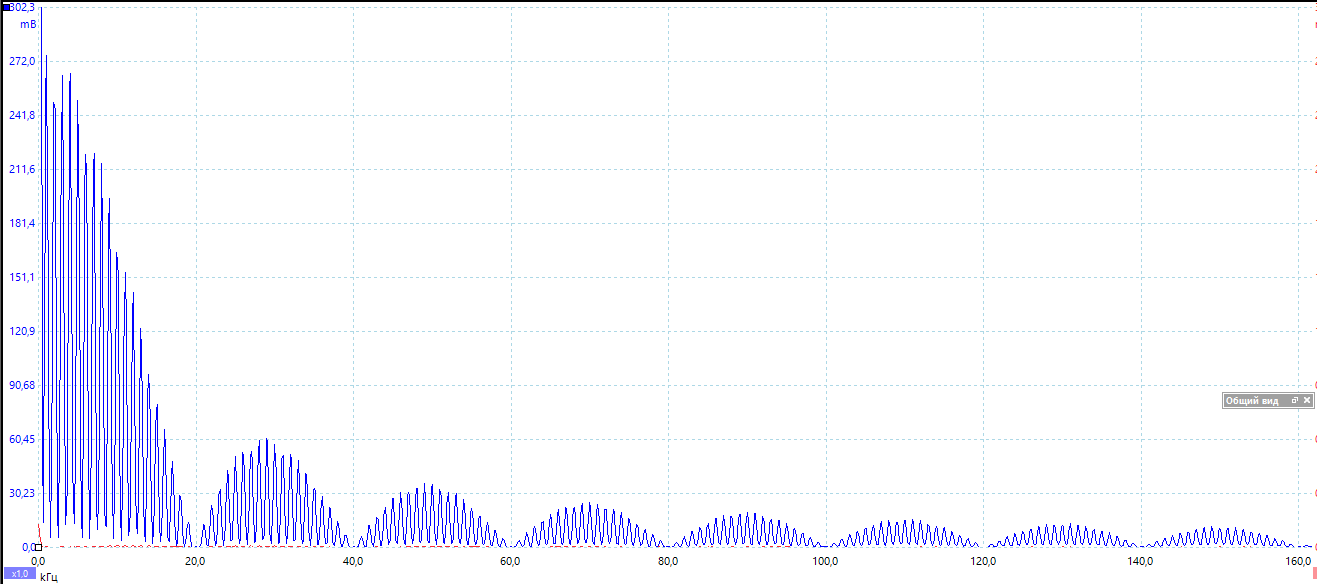
\includegraphics[width=1\linewidth]{б04-407 1 кг 50мкс прямоуг.PNG}} \\ $\nu_\text{повт}$ = 1 кГц
\end{minipage}
\hfill
\begin{minipage}[h]{0.47\linewidth}
\center{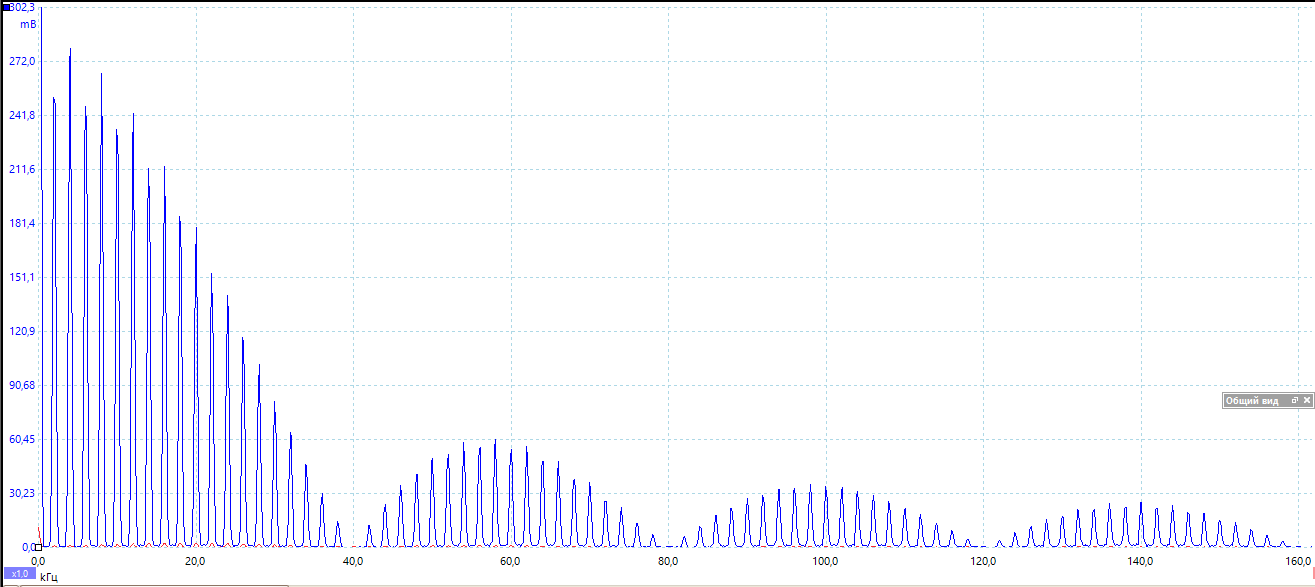
\includegraphics[width=1\linewidth]{б04-407 2 кг 50мкс прямоуг.PNG}} \\ $\nu_\text{повт}$ = 2 кГц
\end{minipage}
\vfill
\begin{minipage}[h]{0.47\linewidth}
\center{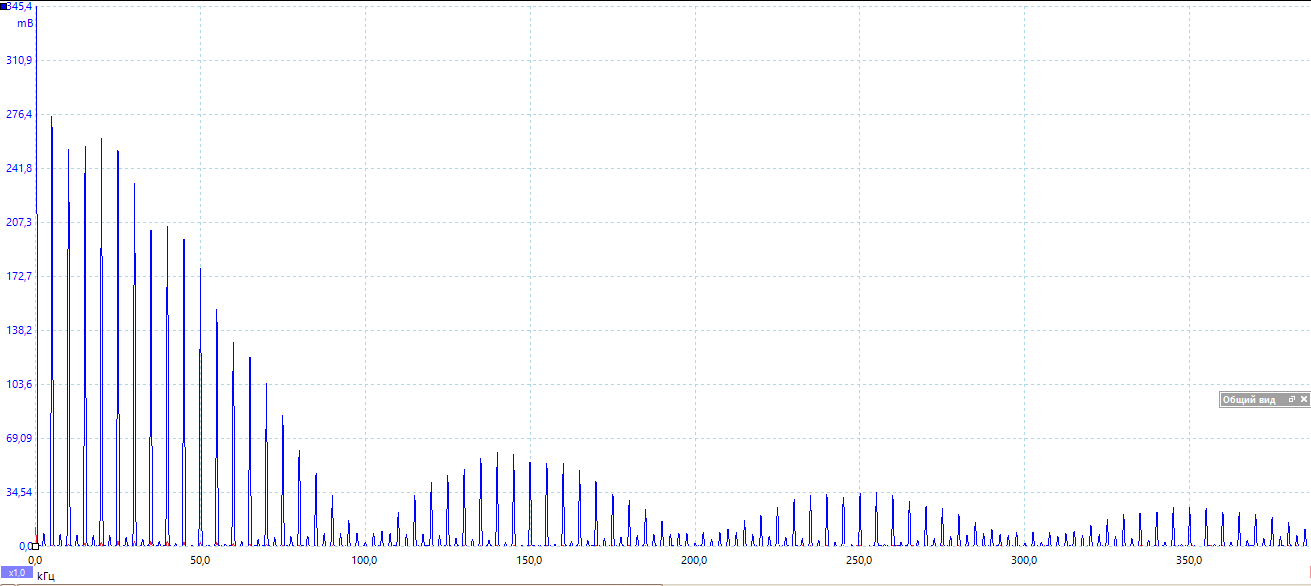
\includegraphics[width=1\linewidth]{б04-407 5кг 50мкс прямоуг.PNG}} \\ $\nu_\text{повт}$ = 5 кГц
\end{minipage}
\hfill
\begin{minipage}[h]{0.47\linewidth}
\center{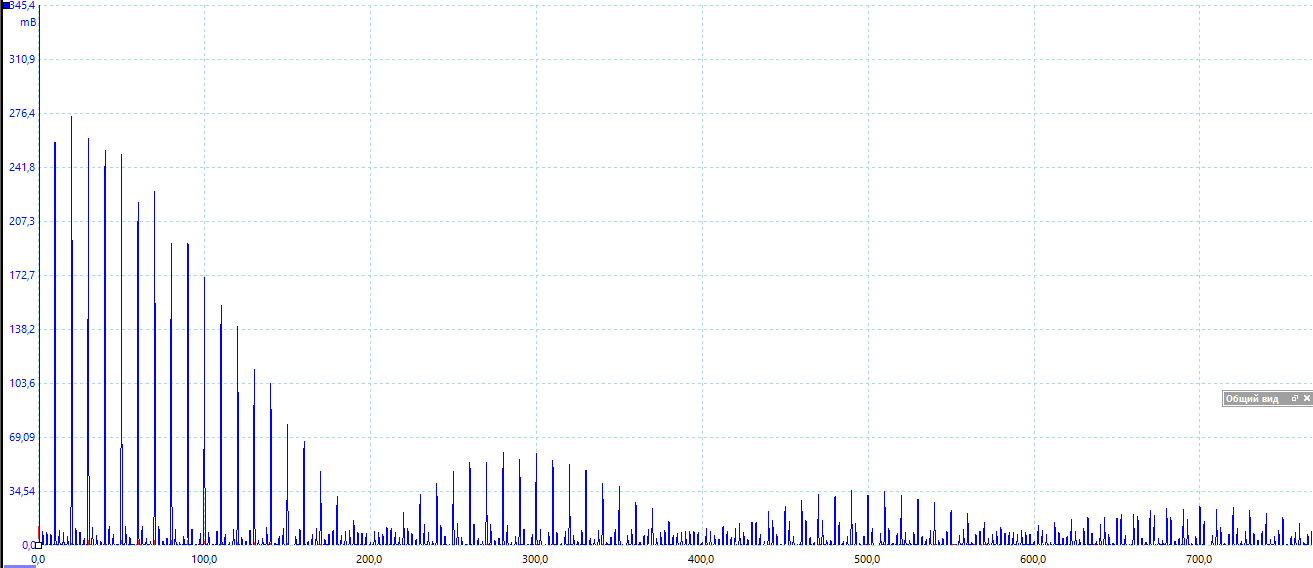
\includegraphics[width=1\linewidth]{б04-407 10кг 50мкс прямоуг.PNG}} \\ $\nu_\text{повт}$ = 10 кГц
\end{minipage}
\caption{Спектры при различных частотах повторения}
\label{ris:experimentalcorrelationsignals}
\end{figure}

Как видно из графиков, при увеличении частоты повторения сигнала увеличивается расстояние между компонентами спектра.

\newpage

\textbf{б.} Изменяем $\tau$ при фиксированном $\nu_\text{повт}$ = 1 кГц и получаем:

\begin{figure}[h]
\begin{minipage}[h]{0.47\linewidth}
\center{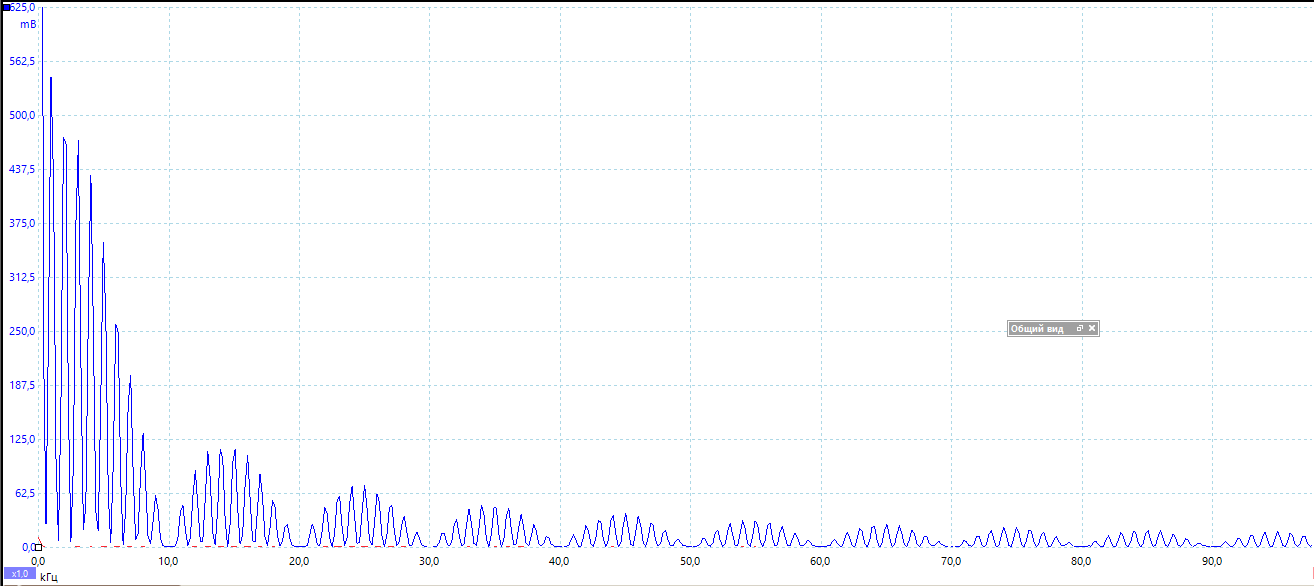
\includegraphics[width=1\linewidth]{б04-407 1кг 100мкс прямоуг.PNG} \\ $\tau$ = 100 мкс
\end{minipage}
\hfill
\begin{minipage}[h]{0.47\linewidth}
\center{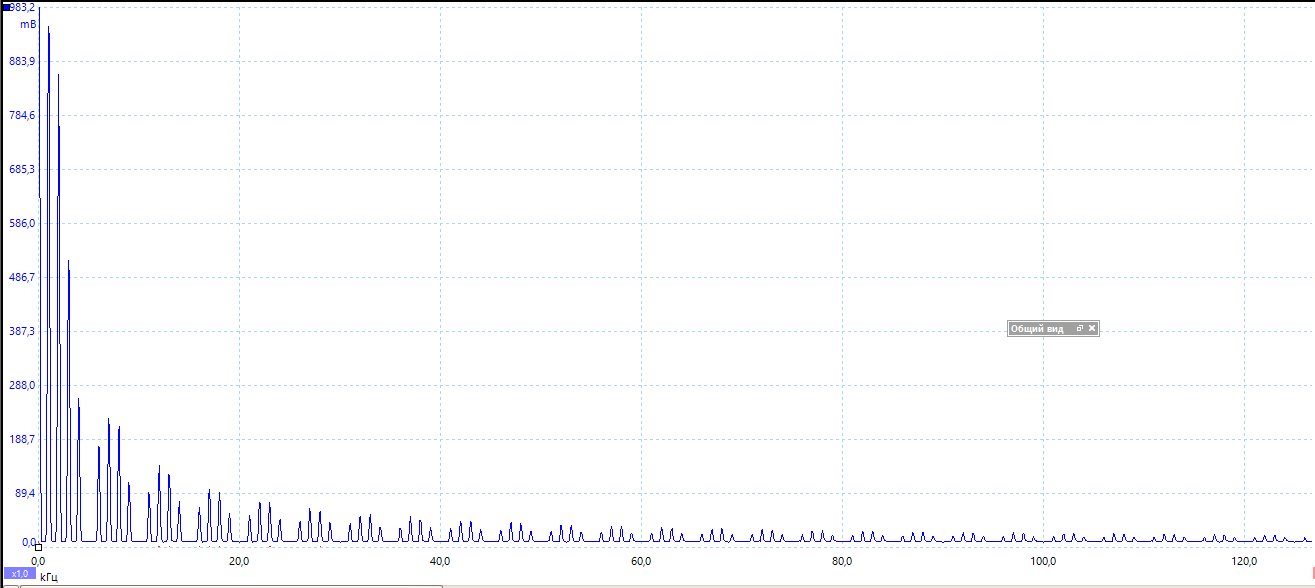
\includegraphics[width=1\linewidth]{б04-407 1кг 200мкс прямоуг.PNG}} \\ $\tau$ = 200 мкс
\end{minipage}
\vfill
\begin{minipage}[h]{0.47\linewidth}
\center{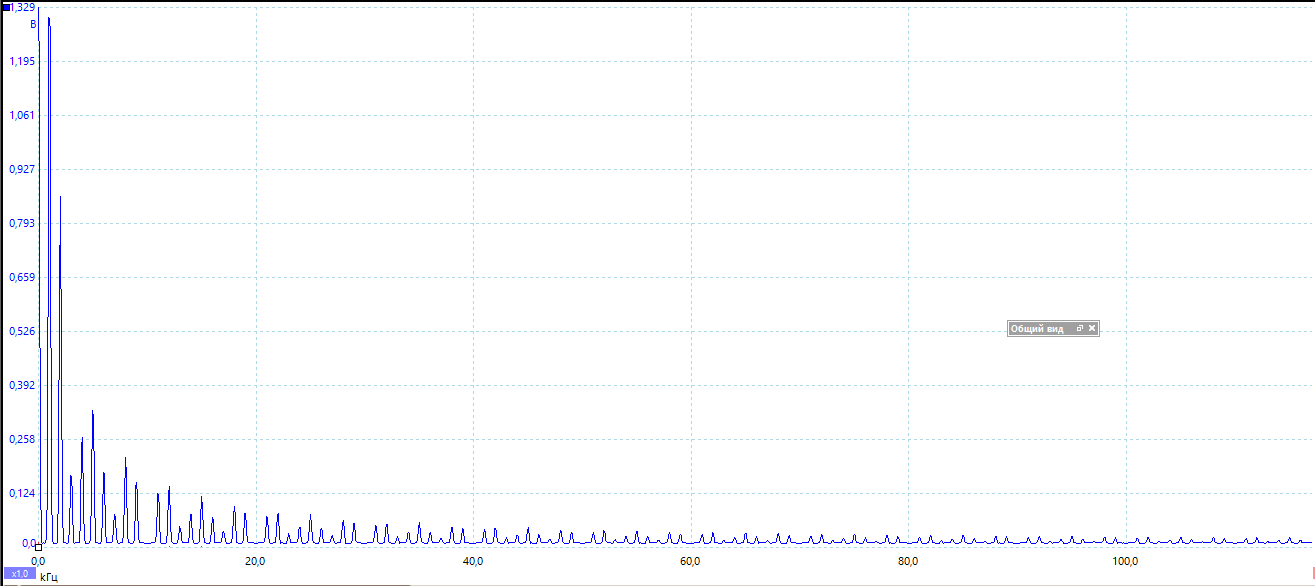
\includegraphics[width=1\linewidth]{б04-407 1кг 300мкс прямоуг.PNG}} \\ $\tau$ = 300 мкс
\end{minipage}
\caption{Спектры при различных длительностях импульса}
\label{ris:experimentalcorrelationsignals2}
\end{figure}

Как видно из графиков, при увеличении длительности сигнала уменьшается ширина спектра.

\item [\textbf{3.}] Измерим амплитуды $a_n$ и частоты $\nu_n$ спектральных гармоник при фиксированных $\nu_\text{повт}$ и $\tau$.

\begin{table}[!h]
\centering
\begin{tabular}{|l|l|l|l|l|l|l|l|l|}
\hline
$n$ гармоники & 5 & 7 & 9 & 11 & 13 & 15 & 17 & 19 \\ \hline
$\nu_n^\text{эксп}$, кГц & 5,025 & 7,013 & 9,028 & 11,00 & 13,02 & 15,01 & 16,99 & 19,00 \\ \hline
$\nu_n^\text{теор}$, кГц & 5 & 7 & 9 & 11 & 13 & 15 & 17 & 19 \\ \hline
$|a_n|^\text{эксп}$, мВ & 252,3 & 219,7 & 192,3 & 155,1 & 112,0 & 77,17 & 42,46 & 12,79 \\ \hline
$|a_n/a_1|_\text{эксп}$ & 0,913 & 0,795 & 0,696 & 0,561 & 0,405 & 0,279 & 0,154 & 0,046 \\ \hline
$|a_n/a_1|_\text{теор}$ & 0,904 & 0,814 & 0,702 & 0,574 & 0,438 & 0,301 & 0,171 & 0,052 \\ \hline
\end{tabular}
\caption{Спектральные гармоники прямоугольного сигнала}
\end{table}

Здесь $a_1 = 276,3$ мВ.
\[
\nu_n^\text{теор} = \frac{n}{T}, \quad |a_n|_\text{теор} = \frac{|\sin(\pi n \tau / T)|}{\pi n}
\]

\item[\textbf{4.}] Зафиксируем период повторения прямоугольного сигнала $T = 1$ мс, $\nu_\text{повт} = 1$ кГц. Изменяя длительность импульса $\tau$ в диапазоне от $\tau=T/50$ до $\tau=T/5$, измерим полную ширину спектра сигнала $\Delta \nu$ — от центра спектра ($\nu = 0$) до гармоники с нулевой амплитудой $a_n \approx 0$ и установим зависимость между $\Delta \nu$ и $\tau$.

\begin{table}[h!]
\centering
\begin{tabular}{|c|c|c|c|c|c|c|c|}
\hline
$\tau$, мкс & 20 & 25 & 40 & 50 & 100 & 150 & 200 \\ \hline
$\Delta \nu$, кГц & 49,95 & 40,04 & 25,02 & 20,00 & 10,03 & 6,645 & 5,015 \\ \hline
$1/\tau \cdot 10^3$, с$^{-1}$ & 50 & 40 & 25 & 20 & 10 & 6,67 & 5 \\ \hline
\end{tabular}
\caption{Исследование зависимости $\Delta \nu$ и $\tau$}
\label{table2}
\end{table}

\begin{figure}[H]
    \centering
    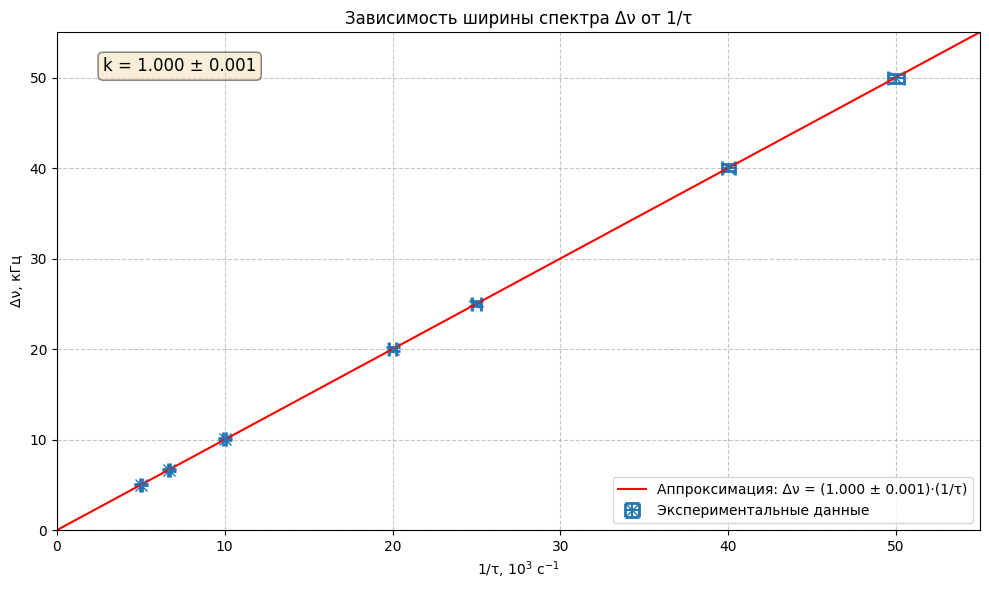
\includegraphics[width=0.9\textwidth]{v by t.png}
    \caption{Зависимость $\Delta\nu$ от $1/\tau$}
    \label{grafic1}
\end{figure}

Построим график $\Delta\nu\left(\frac{1}{\tau}\right)$. Используя МНК, получим $k=0.994\pm0,002$, откуда с хорошей точностью можем заключить, что $\Delta\nu\frac{1}{\tau}=1$, что экспериментально доказывает соотношение неопределённостей.

\item[\textbf{5.}] Зафиксируем длительность импульса прямоугольного сигнала $\tau = 100$ мкс. Изменяя период повторения $T$ в диапазоне от $2\tau$ до $50\tau$ измерим расстояния $\delta\nu = \nu_{n+1} - \nu_n$ между соседними гармониками спектра.

\begin{table}[h!]
\centering
\begin{tabular}{|c|c|c|c|c|c|}
\hline
$\nu$, кГц  & 2 & 1 & 0,5 & 0,25 & 0,1 \\ \hline
$\delta \nu$, кГц & 2,013 & 1,022 & 0,488 & 0,247 & 0,099 \\ \hline
\end{tabular}
\caption{Зависимость $\delta \nu$ от $1/T$}
\label{table3}
\end{table}

\begin{figure}[h!]
    \centering
    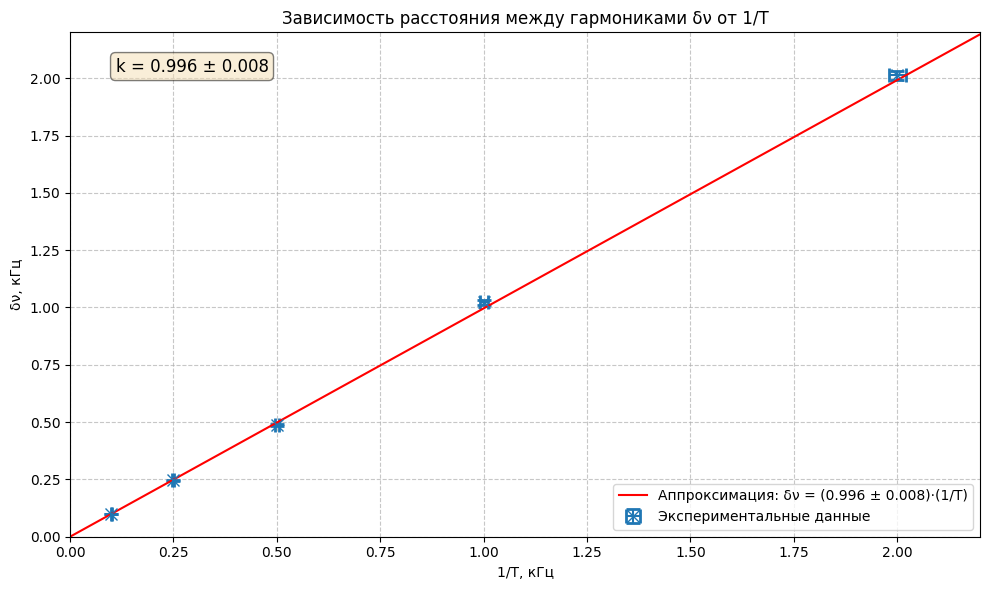
\includegraphics[width=0.9\textwidth]{2 график.png}
    \caption{Зависимость $\delta\nu$ от $1/T$}
    \label{grafic2}
\end{figure}

Построим график $\delta\nu\left(\frac{1}{T}\right)$. Используя МНК, получим $k=0.996\pm0,013$, что экспериментально доказывает соотношение неопределённостей. График приведён на рис.13.
\end{enumerate}

\newpage

\subsection*{Б. Наблюдение спектра периодической последовательности цугов}

\begin{enumerate}
\item [\textbf{1.}] Настраиваем генератор на периодичные импульсы синусоидальной формы (цугов) с несущей частотой $\nu_0$ = 50 кГц, частотой повторения $\nu_\text{повт}$ = 1 кГц, число периодов синусоиды в одном импульсе $N$ = 5 (что соответствует длительности импульса $\tau$ = $N/\nu_o$ = 100 мкс).

\item [\textbf{2.}] Получаем на экране спектр (Преобразование Фурье) сигнала.

\textbf{a.} Изменяем $N$ при фиксированных $\nu_0$ = 50 кГц и $\nu_\text{повт}$ = 1 кГц:

\begin{figure}[h]
\begin{minipage}[h]{0.47\linewidth}
\center{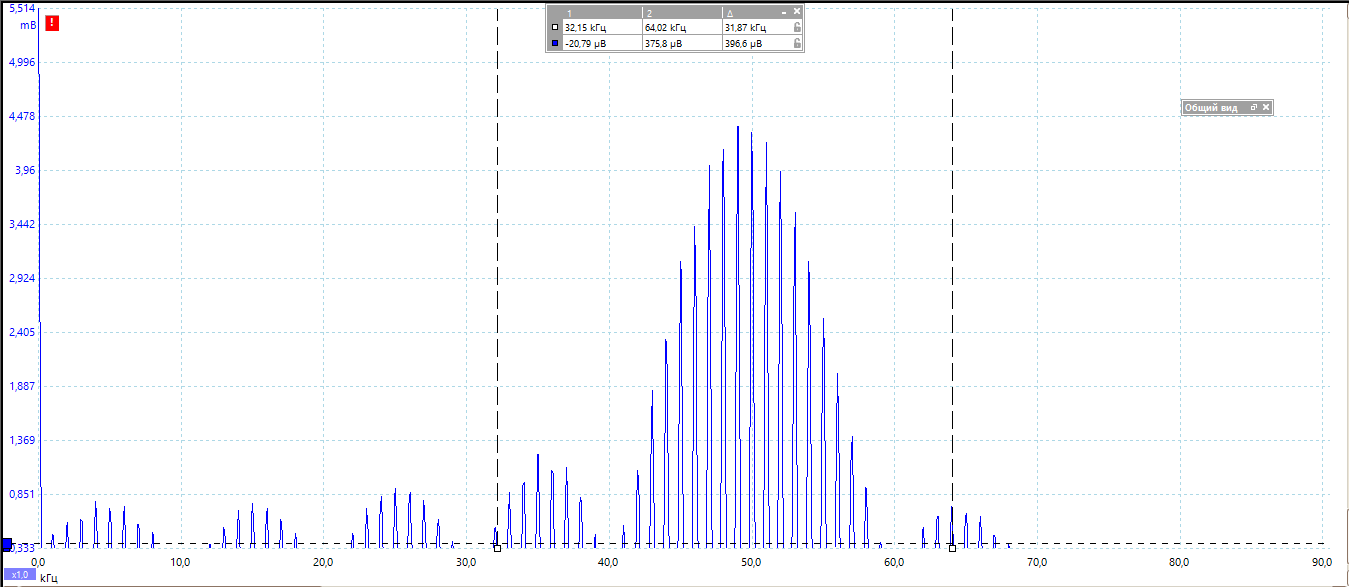
\includegraphics[width=1\linewidth]{б04-407 пункт Б 5Н.PNG}} \\ N=5, $\delta \nu$ = 1 кГц, $\Delta \nu$ = 10 кГц
\end{minipage}
\hfill
\begin{minipage}[h]{0.47\linewidth}
\center{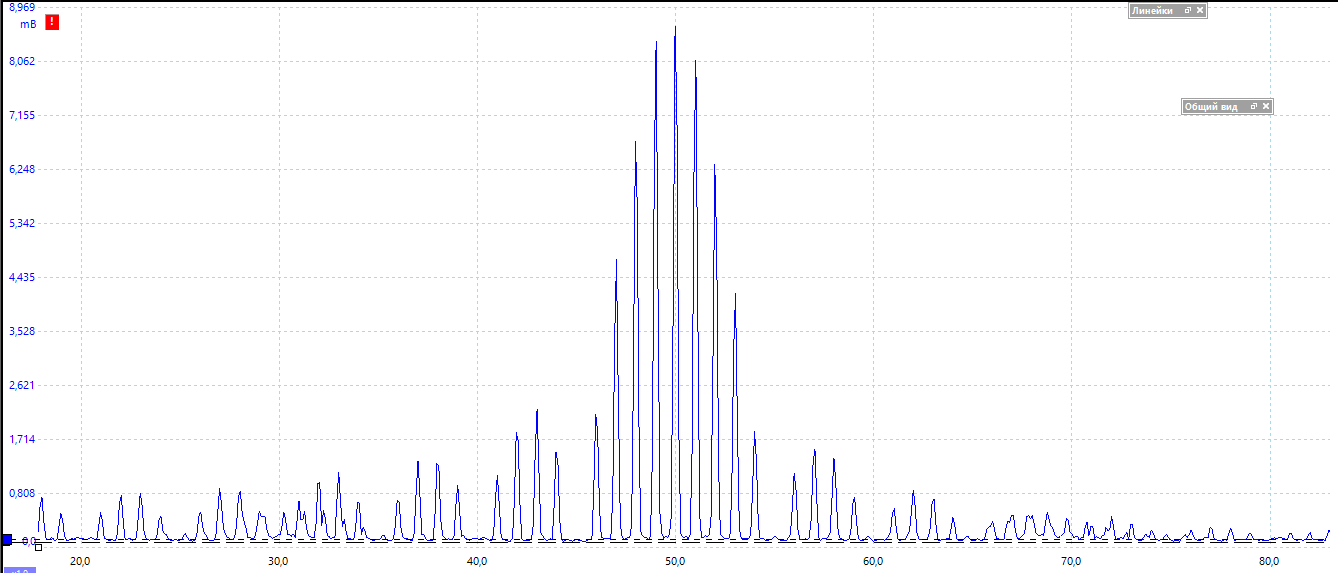
\includegraphics[width=1\linewidth]{б04-407 пункт Б 10Н.PNG}} \\ N=10, $\delta \nu$ = 1 кГц, $\Delta \nu$ = 5 кГц
\end{minipage}
\vfill
\begin{minipage}[h]{0.47\linewidth}
\center{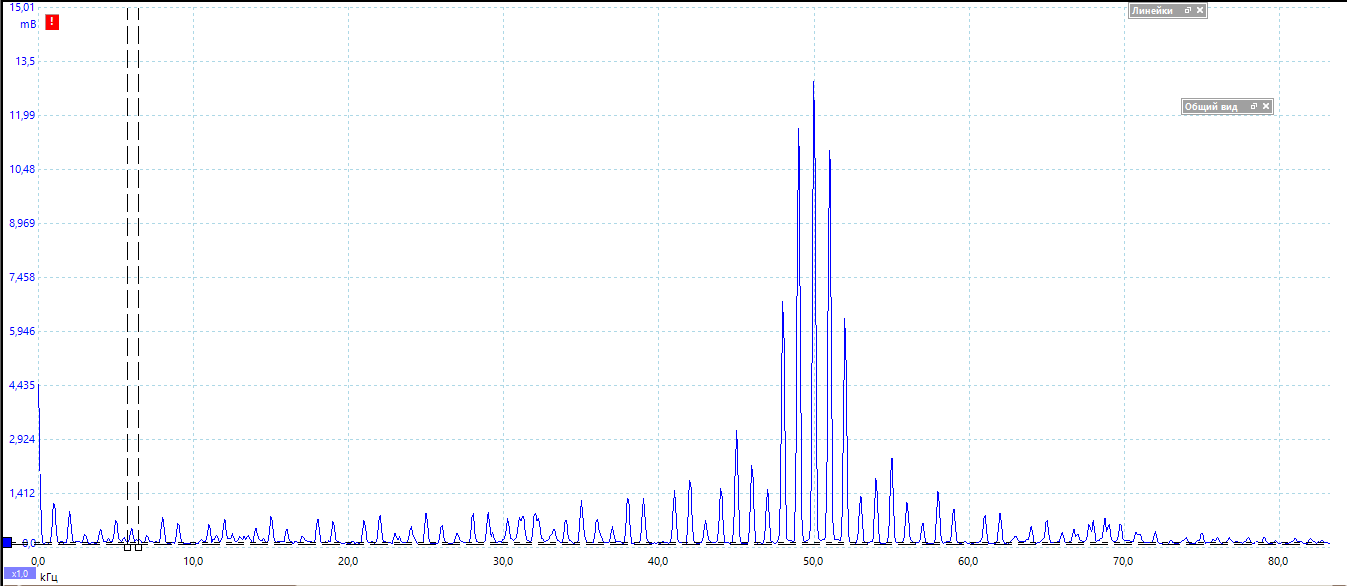
\includegraphics[width=1\linewidth]{б04-407 пункт Б 15Н.PNG}} \\ N=15, $\delta \nu$ = 1 кГц, $\Delta \nu$ $\approx$ 3 кГц
\end{minipage}
\hfill
\begin{minipage}[h]{0.47\linewidth}
\center{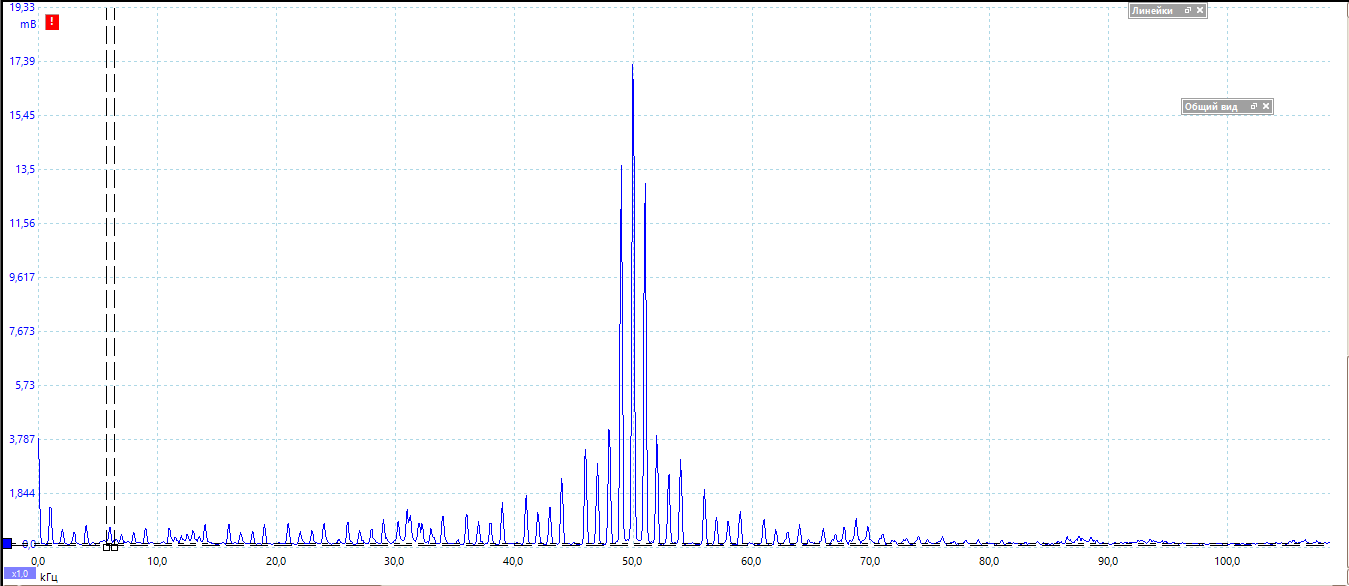
\includegraphics[width=1\linewidth]{б04-407 пункт Б 20Н.PNG}} \\ N=20, $\delta \nu$ = 1 кГц, $\Delta \nu$ $\approx$ 2.5 кГц
\end{minipage}
\caption{Спектры цугов при различном количестве периодов}
\label{ris:experimentalcorrelationsignals3}
\end{figure}

Соотношение неопределённостей:
\[
\Delta \nu \cdot \tau = 10\cdot10^3\cdot\frac{5}{50\cdot10^3} = 5\cdot10^3\cdot\frac{10}{50\cdot10^3} = 2.5\cdot10^3\cdot\frac{20}{50\cdot10^3} \approx 3\cdot10^3\cdot\frac{15}{50\cdot10^3} \approx 1
\]

Видим, что спектр остаётся симметричным относительно одной и той же точки, однако "сжимается" к ней при увеличении N.

\newpage

\textbf{б.} Изменяем $\nu_0$ при фиксированных N = 5 и $\nu_\text{повт}$ = 1 кГц:

\begin{figure}[h]
\begin{minipage}[h]{0.47\linewidth}
\center{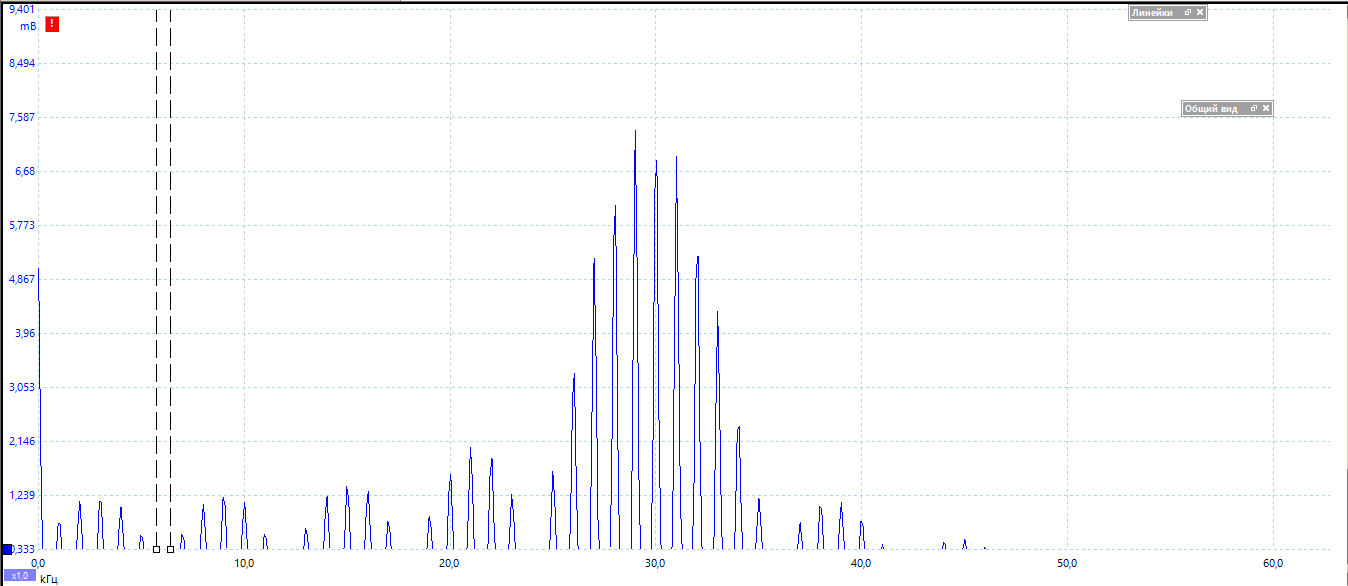
\includegraphics[width=1\linewidth]{б04-407 пункт Б 30кГц 5н.PNG}} \\ $\nu_0$ = 30 кГц, $\delta \nu$ = 1 кГц, $\Delta \nu$ = 6 кГц
\end{minipage}
\hfill
\begin{minipage}[h]{0.47\linewidth}
\center{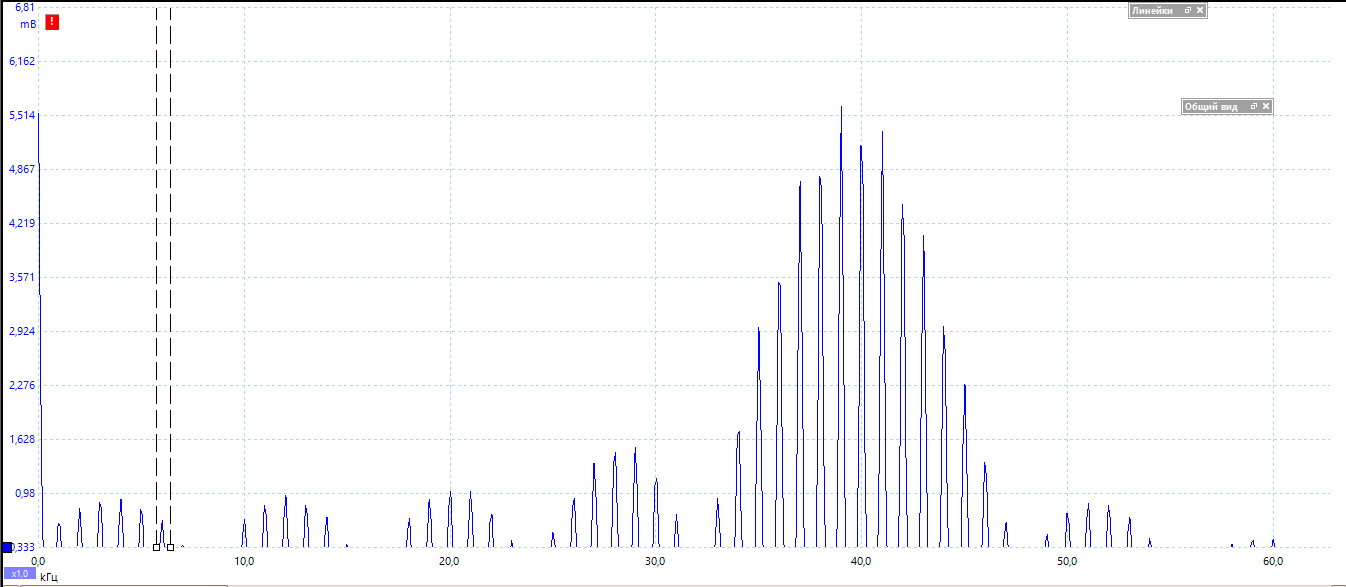
\includegraphics[width=1\linewidth]{б04-407 пункт Б 40кгц 5н.PNG}} \\ $\nu_0$ = 40 кГц, $\delta \nu$ = 1 кГц, $\Delta \nu$ = 8 кГц
\end{minipage}
\vfill
\begin{minipage}[h]{0.47\linewidth}
\center{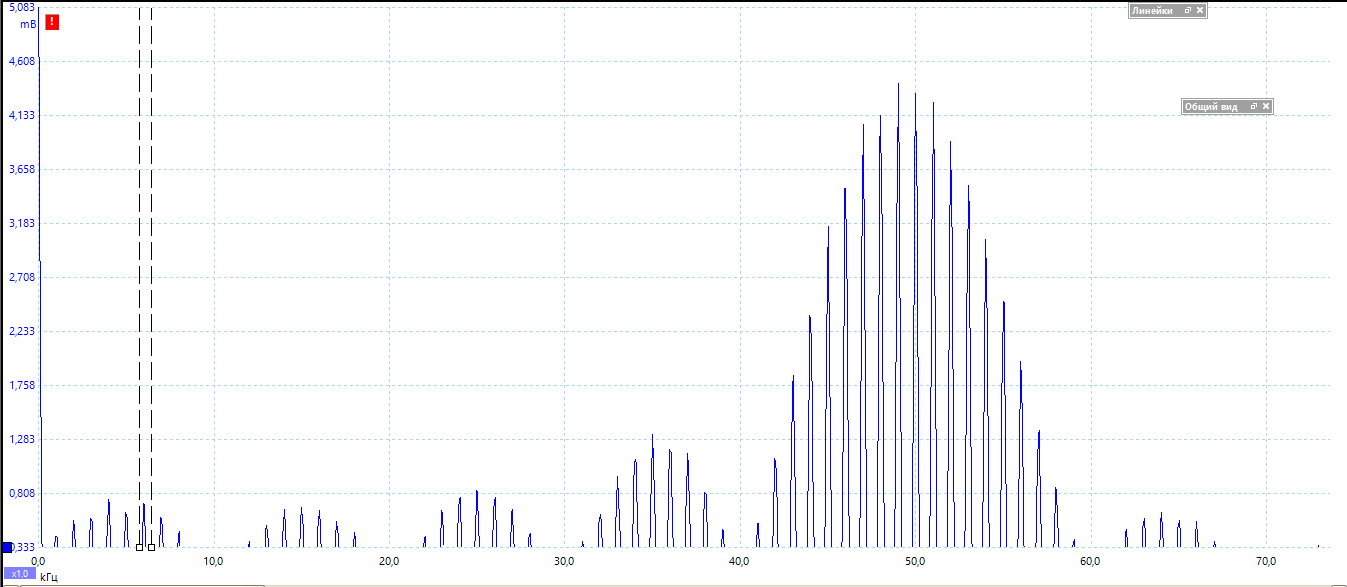
\includegraphics[width=1\linewidth]{б04-407 пункт Б 50кгц 5н.PNG}} \\ $\nu_0$ = 50 кГц, $\delta \nu$ = 1 кГц, $\Delta \nu$ = 10 кГц
\end{minipage}
\caption{Спектры цугов при различных несущих частотах}
\label{ris:experimentalcorrelationsignals4}
\end{figure}

Соотношение неопределённостей:
\[
\Delta \nu \cdot \tau = 6\cdot10^3\cdot\frac{5}{30\cdot10^3} = 8\cdot10^3\cdot\frac{5}{40\cdot10^3} = 10\cdot10^3\cdot\frac{5}{50\cdot10^3} = 1
\]

Видим, что в этом случае спектр не меняет свою форму, однако его центр смещается в соответсвии с изменением частоты несущей.

\newpage

\textbf{в.} Изменяем $\nu_\text{повт}$ при фиксированных N = 5 и $\nu_0$ = 50 кГц:

\begin{figure}[h]
\begin{minipage}[h]{0.47\linewidth}
\center{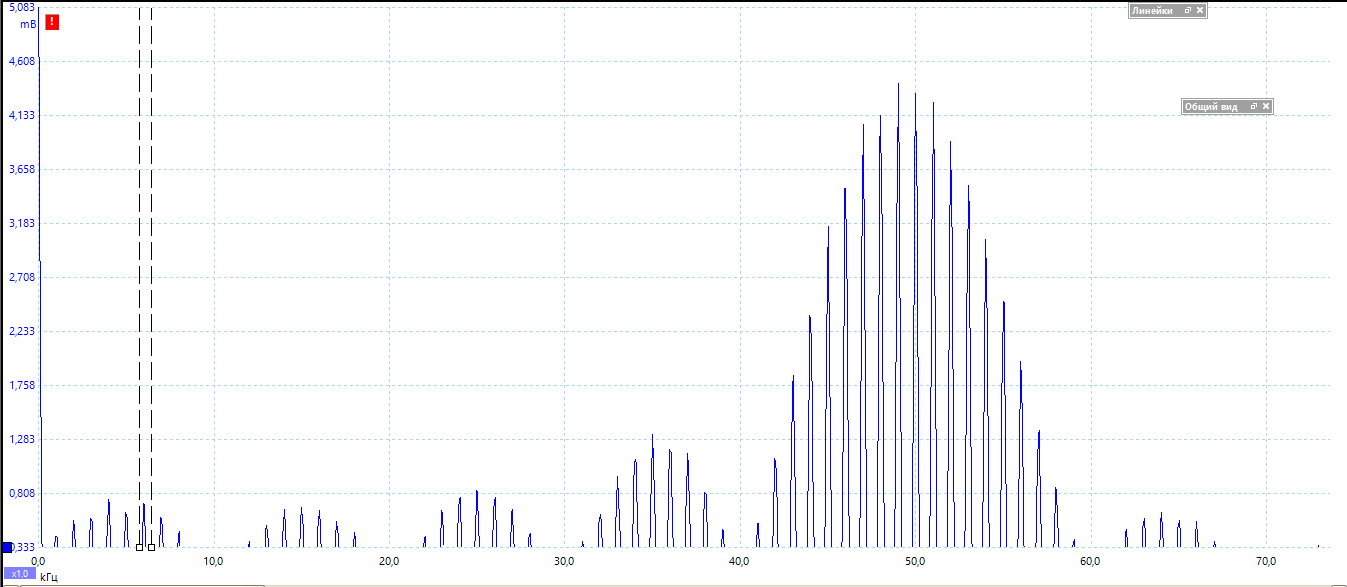
\includegraphics[width=1\linewidth]{б04-407 пункт Б 50кгц 5н.PNG}} \\ $\nu_\text{повт}$ = 1 кГц, $\delta \nu$ = 1 кГц, $\Delta \nu$ = 10 кГц
\end{minipage}
\hfill
\begin{minipage}[h]{0.47\linewidth}
\center{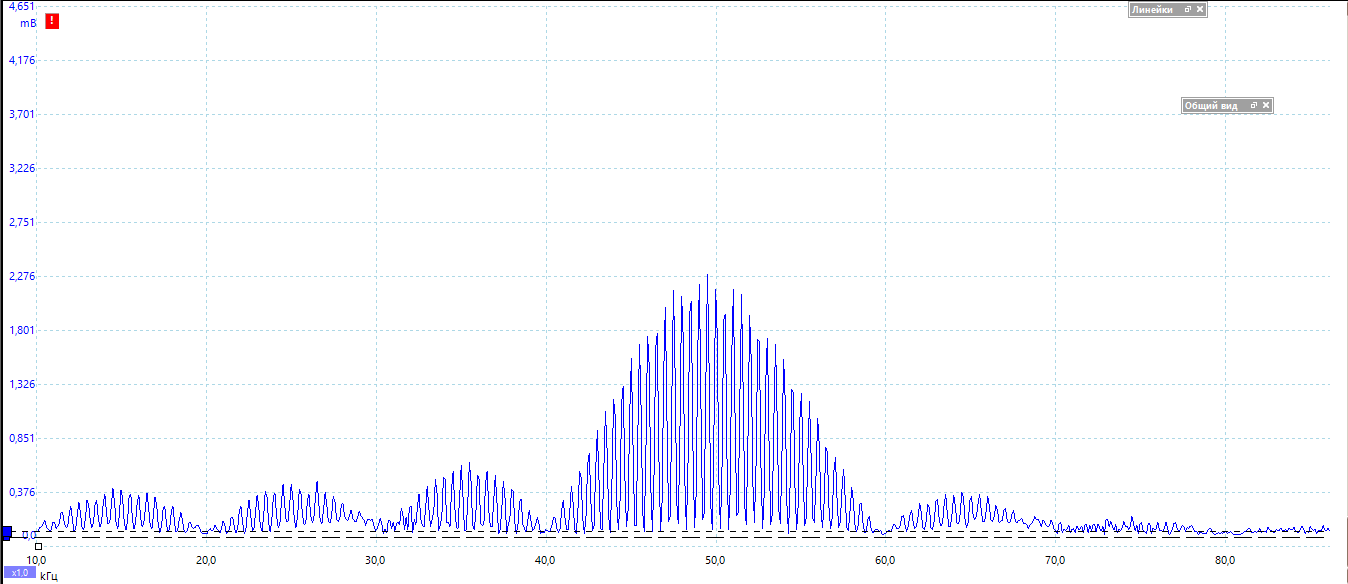
\includegraphics[width=1\linewidth]{б04-407 пункт Б 50кгц 2мс.PNG}} \\ $\nu_\text{повт}$ = 0.5 кГц, $\delta \nu$ = 0.5 кГц, $\Delta \nu$ = 10 кГц
\end{minipage}
\vfill
\begin{minipage}[h]{0.47\linewidth}
\center{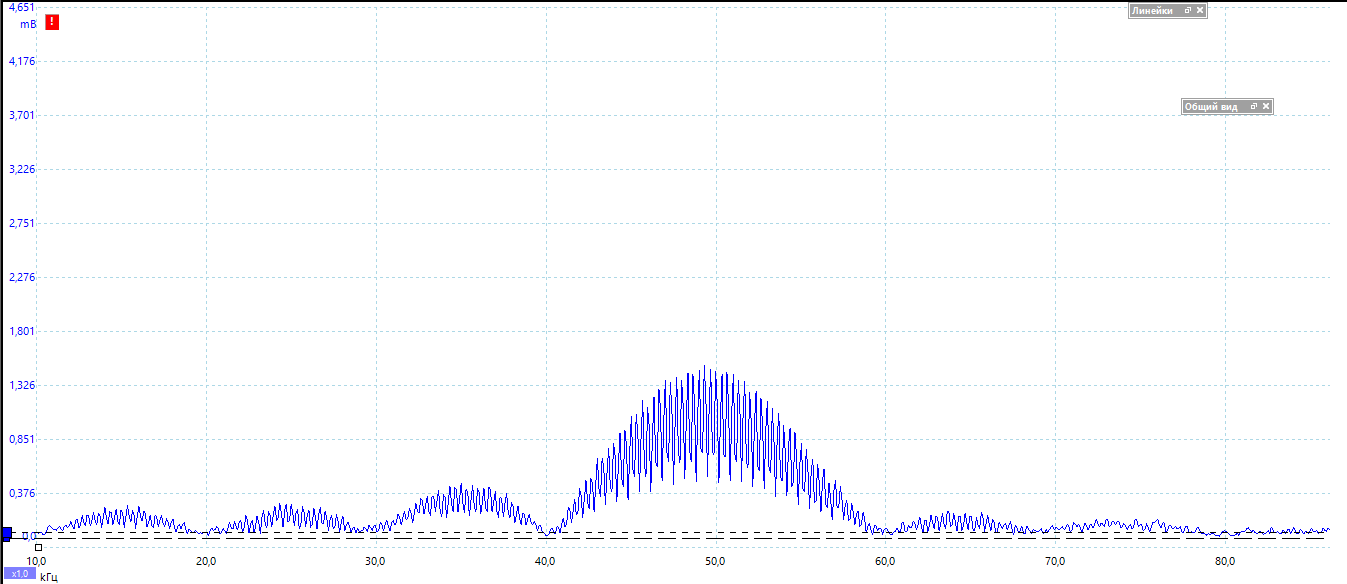
\includegraphics[width=1\linewidth]{б04-407 пункт Б 50кгц 3мс.PNG}} \\ $\nu_\text{повт}$ = 0.25 кГц, $\delta \nu$ = 0.25 кГц, $\Delta \nu$ = 10 кГц
\end{minipage}
\caption{Спектры цугов при различных частотах повторения}
\label{ris:experimentalcorrelationsignals5}
\end{figure}

Видно, что соотношение неопределённости выполняется:
\[
\frac{\delta \nu}{\nu_\text{повт}} = \frac{1\cdot10^3}{1\cdot10^3} = \frac{0.5\cdot10^3}{0.5\cdot10^3} = \frac{0.25\cdot10^3}{0.25\cdot10^3} = 1
\]

Также видно, что при стремлении частоты повторения к нулю, стремится к нулю и расстояние между компонентами спектра.
\end{enumerate}

\newpage

\subsection*{Г. Наблюдение спектра амплитудно-модулированного сигнала}

\begin{enumerate}
\item [\textbf{1.}] Настраиваем генератор в режим модулированного по амплитуде синусоидального сигнала с несущей частотой $\nu_0$ = 50 кГц, частотой модуляции $\nu_\text{мод}$ = 2 кГц и глубиной модуляции $m$ = 0.5.

\item [\textbf{2.}] Получаем на экране спектр (Преобразование Фурье) сигнала. Из графика получим $A_{max} = 3.057$ мВ и $A_{min} = 1.027$ мВ и убедимся в справедливости соотношения 
\[
m = \frac{A_\text{max} - A_\text{min}}{A_\text{max} + A_\text{min}} = \frac{2.03}{4.084} \approx 0.5
\]
Поскольку мы установили глубину модуляции на $0,5$, а из теории у нас получилась $0,497$, то мы видим, что формула верна.

\item [\textbf{3.}] Изменяя на генераторе глубину модуляции $m$ в диапазоне от 10 \% до 100 \%, измерим отношение амплитуд боковой и основной спектральных линий $a_{\text{бок}}/a_{\text{осн}}$. Построим график зависимости $a_{\text{бок}}/a_{\text{осн}}$ от $m$ и проверим, совпадает ли результат с теоретическим.

\begin{center}
\begin{tabular}{|c|c|c|c|c|c|c|c|}
\hline
$m$, \% & 10 & 20 & 30 & 40 & 50 & 80 & 100 \\ \hline
$a_{\text{бок}}$, мВ & 27,76 & 57,03 & 82,4 & 109,7 & 140,9 & 222,9 & 279,5 \\ \hline
\multicolumn{8}{|c|}{$a_{\text{осн}}$ = 566,3 мВ} \\ \hline
$a_{\text{бок}}/a_{\text{осн}}$ & 0,049 & 0,101 & 0,145 & 0,194 & 0,249 & 0,394 & 0,494 \\ \hline
\end{tabular}

\textbf{Таблица 4.} Исследование зависимости $a_{\text{бок}}/a_{\text{осн}}$ от $m$.
\end{center}

\begin{figure}[h!]
    \centering
    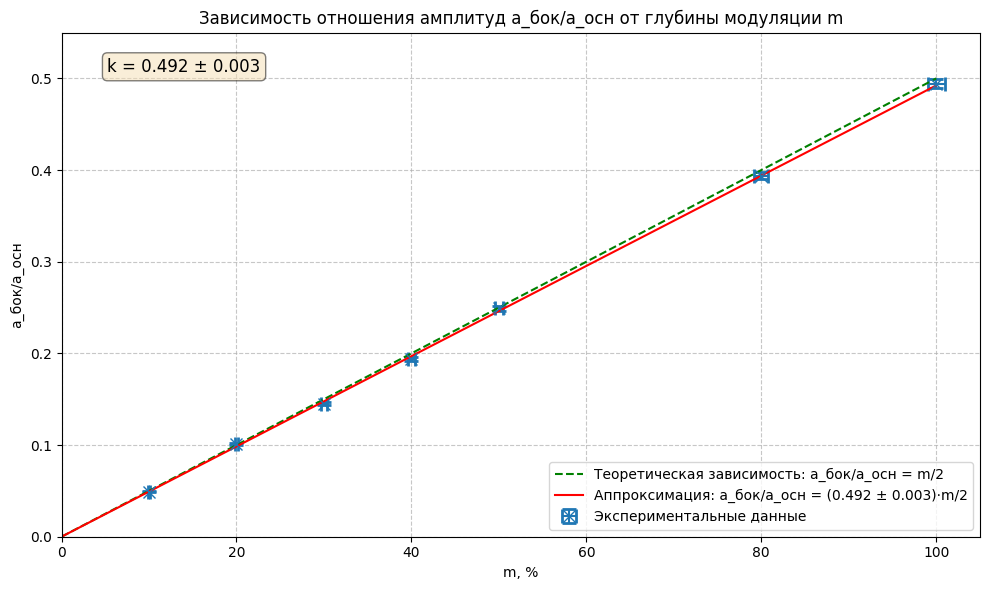
\includegraphics[width=0.9\textwidth]{график 3.png}
    \caption{Зависимость отношения амплитуд $a_{\text{бок}}/a_{\text{осн}}$ от глубины модуляции $m$}
    \label{grafic3}
\end{figure}

Построим график $\frac{a_{\text{бок}}}{a_{\text{осн}}}(m)$. Используя МНК, получим $k=0.516x\pm0,00007$, что подтверждает $\frac{a_{\text{бок}}}{a_{\text{осн}}}=\frac{m}{2}$, т.е. совпадает с теоретическим предсказанием. График приведён на рис.\ref{grafic3}.
\end{enumerate}

\newpage

\subsection*{Д. Наблюдение спектра сигнала, модулированного по фазе}

\begin{enumerate}
\item [\textbf{1.}] Настраиваем генератор в режим модулированного по фазе синусоидального сигнала с несущей частотой $\nu_0$ = 50 кГц, частотой модуляции $\nu_\text{мод}$ = 2 кГц и максимальным отклонением $\varphi$ = 10$\degree$.

\item [\textbf{2.}] Получаем на экране спектр (Преобразование Фурье) сигнала.

\begin{figure}[h]
\begin{minipage}[h]{0.44\linewidth}
\center{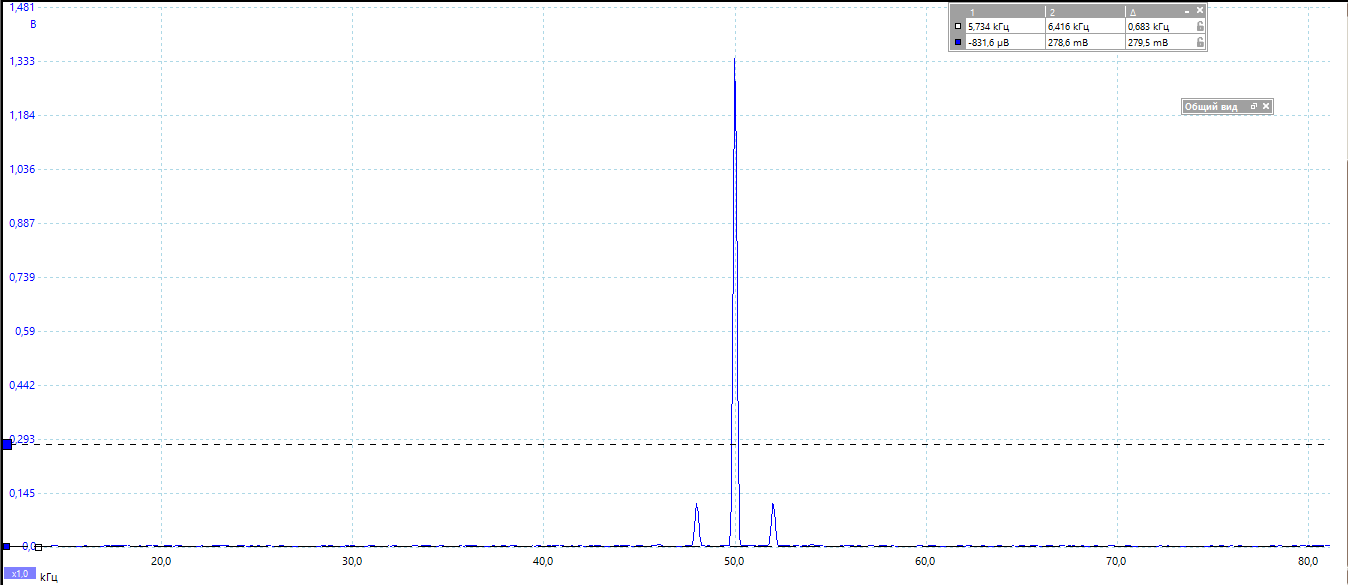
\includegraphics[width=1\linewidth]{б04-407 пунктД 2кгц мод 50кгц нес 10град.PNG}} \\ $\nu_0$ = 50 кГц, $\nu_\text{мод}$ = 2 кГц, $\varphi$ = 10$\degree$
\end{minipage}
\hfill
\begin{minipage}[h]{0.44\linewidth}
\center{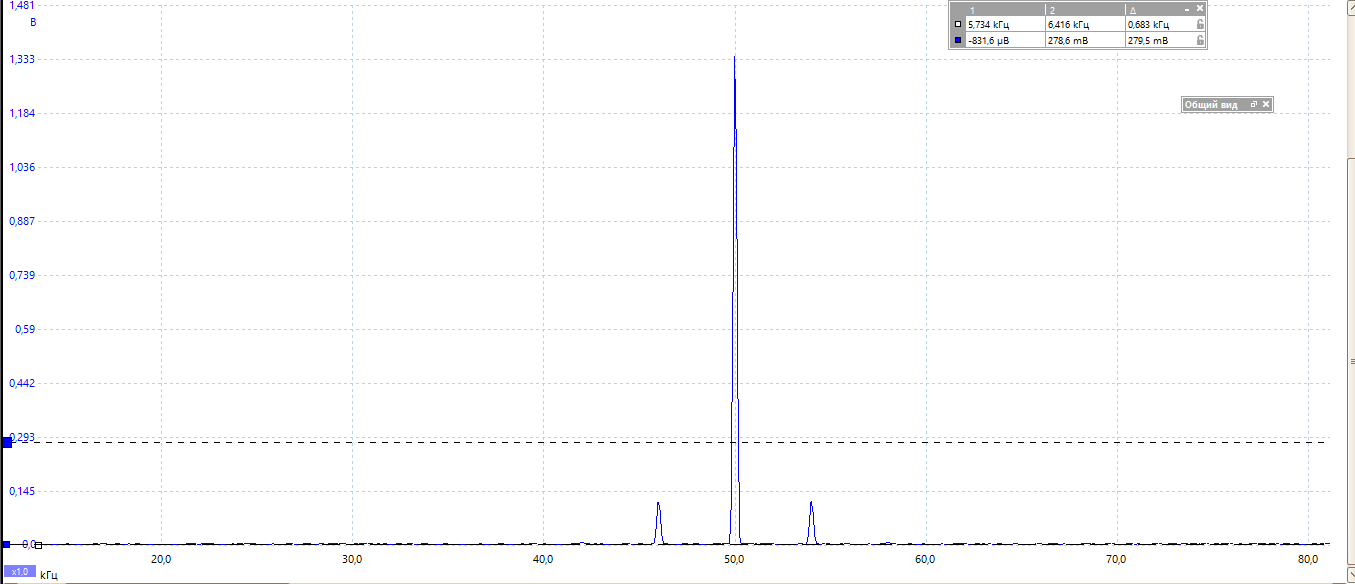
\includegraphics[width=1\linewidth]{б04-407 пунктД 3гкц мод 50кгц нес 10град.PNG} \\ $\nu_0$ = 50 кГц, $\nu_\text{мод}$ = 3 кГц, $\varphi$ = 10$\degree$
\end{minipage}
\vfill
\begin{minipage}[h]{0.44\linewidth}
\center{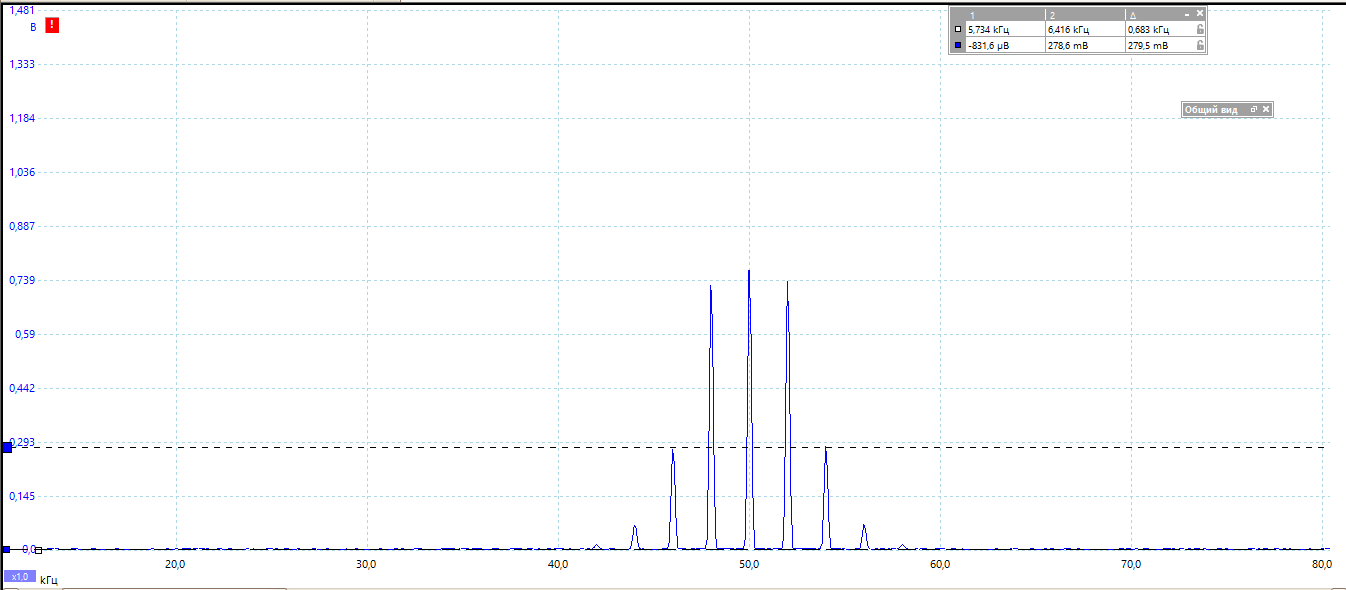
\includegraphics[width=1\linewidth]{б04-407 пунктД 2кгц мод 50кгц нес 80град.PNG}} \\ $\nu_0$ = 50 кГц, $\nu_\text{мод}$ = 2 кГц, $\varphi$ = 80$\degree$
\end{minipage}
\hfill
\begin{minipage}[h]{0.44\linewidth}
\center{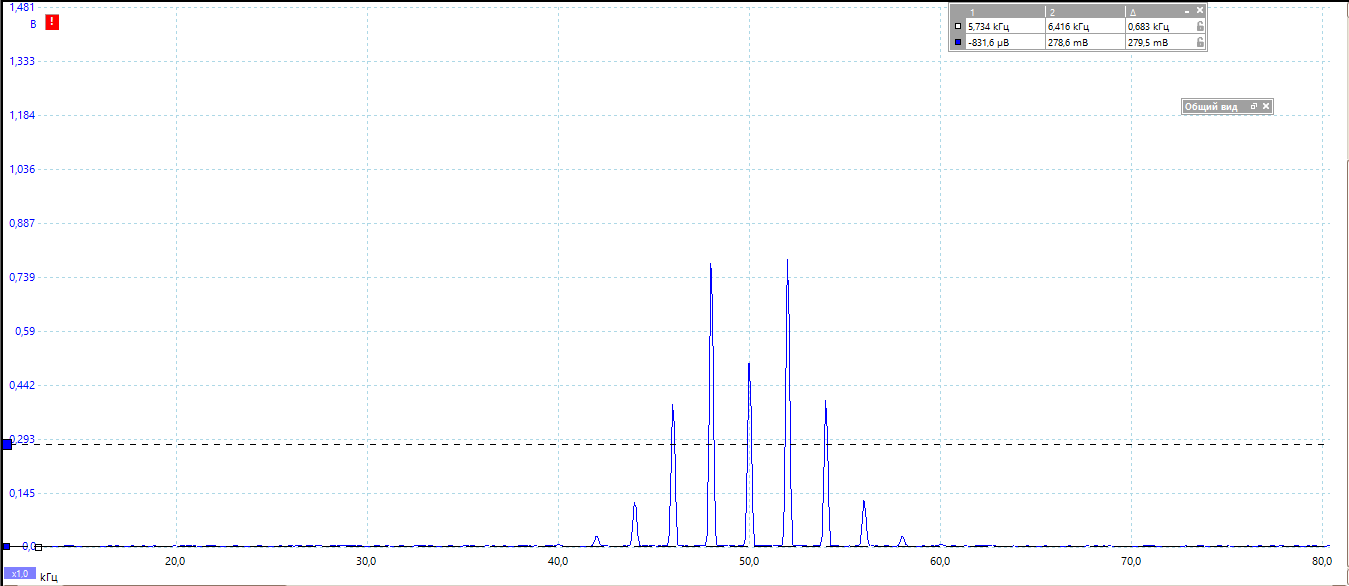
\includegraphics[width=1\linewidth]{б04-407 пунктД 2кгц мод 50кгц нес 100град.PNG}} \\ $\nu_0$ = 50 кГц, $\nu_\text{мод}$ = 2 кГц, $\varphi$ = 100$ \degree$
\end{minipage}
\vfill
\caption{Спектры фазо-модулированных сигналов}
\label{ris:experimentalcorrelationsignals6}
\end{figure}

\newpage

\begin{figure}[h]
\begin{minipage}[h]{0.44\linewidth}
\center{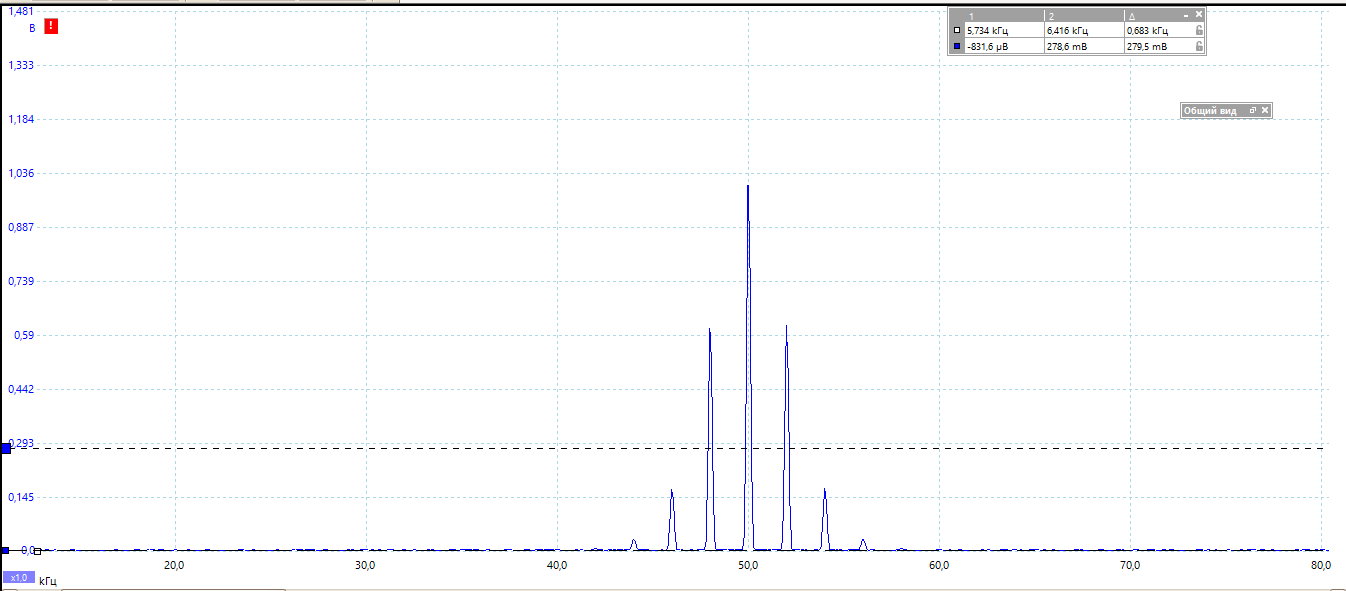
\includegraphics[width=1\linewidth]{б04-407 пунктД 2кгц 50кгц нес 60град.PNG}} \\ $\nu_0$ = 50 кГц, $\nu_\text{мод}$ = 2 кГц, $\varphi$ = 60$ \degree$
\end{minipage}
\caption{Спектр фазо-модулированного сигнала}
\label{ris:experimentalcorrelationsignals7}
\end{figure}
\end{enumerate}

\subsection*{Е. Исследование RC-фильтра низких частот}

\begin{enumerate}
\item [\textbf{1.}] Для RC-цепочки с параметрами $R$ и $C$ характерное время определяется выражением
\[
\tau_{RC} = R \cdot C.
\]
В эксперименте использовался прямоугольный сигнал с периодом повторения 
\[
T = 300\ \mu\text{с}.
\]

\item [\textbf{2.}] Собираем схему согласно методическим указаниям. На вход RC-цепочки подаём последовательность прямоугольных импульсов с периодом $T$ и длительностью $\tau = T/20$. С помощью осциллографа регистрируем спектр сигнала до и после фильтра.

\item [\textbf{3.}] Для каждой гармоники измеряем амплитуды исходного ($a_n^{(0)}$) и фильтрованного ($a_n^{(f)}$) сигналов. Рассчитываем коэффициенты фильтрации по формуле:
\[
K_n = \frac{a_n^{(f)}}{a_n^{(0)}},
\]
а также их погрешности
\[
\Delta K_n = K_n \cdot \sqrt{\left(\frac{\Delta a_n^{(f)}}{a_n^{(f)}}\right)^2 + \left(\frac{\Delta a_n^{(0)}}{a_n^{(0)}}\right)^2}.
\]

\begin{table}[h!]
\centering
\begin{tabular}{|c|c|c|c|c|c|}
\hline
$n$ & $a_n^{(0)}$, усл. ед. & $a_n^{(f)}$, усл. ед. & $\frac{a_n^{(0)}}{a_n^{(f)}}$ & $K_n^{\text{эксп}}$ & $\Delta K_n$ \\ \hline
1 & 63.18 & 62.98 & 1.003 &0.997 & 0.014 \\ \hline
2 & 69.51 & 69.31 & 1.003 & 0.997 & 0.014 \\ \hline
3 & 62.30 & 61.92 & 1.006 & 0.994 & 0.014 \\ \hline
4 & 58.49 & 58.93 & 0.992 & 1.008 & 0.014 \\ \hline
5 & 54.74 & 54.01 & 1.013 & 0.987 & 0.014 \\ \hline
6 & 45.94 & 45.74 & 1.004 & 0.996 & 0.014 \\ \hline
7 & 43.30 & 43.10 & 1.005 & 0.995 & 0.014 \\ \hline
8 & 39.61 & 38.97 & 1.016 & 0.984 & 0.014 \\ \hline
9 & 34.68 & 34.13 & 1.016 & 0.984 & 0.014 \\ \hline
\end{tabular}
\caption{Амплитуды гармоник и коэффициенты фильтрации}
\label{tab:RC}
\end{table}

\item [\textbf{4.}] Строим график зависимости коэффициента фильтрации $K(\nu)$ от частоты.

\begin{figure}[H]
    \centering
    \begin{tikzpicture}
        \begin{axis}[
            xlabel={Частота \(\nu\), кГц},
            ylabel={Коэффициент фильтрации \(K\)},
            xmin=0, xmax=35,
            ymin=0.97, ymax=1.02,
            grid=both,
            width=0.9\textwidth,
            height=0.6\textwidth,
            legend pos=north east,
        ]
        \addplot+[
            only marks,
            error bars/.cd,
            y dir=both,
            y explicit,
        ]
        table[
            x=nu,
            y=K,
            y error=deltaK,
        ] {
            nu      K       deltaK
            3.333   0.997   0.014
            6.667   0.997   0.014
            10.000  0.994   0.014
            13.333  1.008   0.014
            16.667  0.987   0.014
            20.000  0.996   0.014
            23.333  0.995   0.014
            26.667  0.984   0.014
            30.000  0.984   0.014
        };
        \addlegendentry{Эксперимент (точки)};

        \addplot[green, thick, domain=0:30, samples=200] {1/sqrt(1 + (2*pi*x*0.948925*1e-3)^2)};
        \addlegendentry{Аппрокс. ( $\tau_{RC} = 0.9489\ \mu\text{s}$ )};


        \addplot[red, thick, domain=0:30, samples=100] {1/sqrt(1 + (2*pi*x*1e-3)^2)};
        \addlegendentry{Теория ( $\tau_{RC} = 1\ \mu\text{s}$ )};
        \end{axis}
    \end{tikzpicture}
    \caption{Зависимость коэффициента фильтрации \(K(\nu)\): экспериментальные данные, аппроксимация и теоретическая кривая}
    \label{grafic4}
\end{figure}

\item [\textbf{5.}] Поиск параметра аппроксимационной кривой.

\begin{enumerate}
  \item Модель аппроксимации :
  \[
  K(\nu;\tau)=\frac{1}{\sqrt{1 + \bigl(2\pi\nu\tau\bigr)^2}}.
  \]
  Здесь частота \(\nu\) дана в килогерцах (кГц) в таблице; при подстановке в численные выражения использовали перевод в герцы: \(\nu[\text{Гц}]=\nu[\text{кГц}]\times 10^3\).

  \item Критерий качества аппроксимации (взвешенный МНК, критерий $\chi^2$):
  \[
  \chi^2(\tau)=\sum_{i=1}^{N}\left(\frac{K^{\text{(exp)}}_i - K(\nu_i;\tau)}{\Delta K_i}\right)^2,
  \]
  где $N=9$ — число гармоник, $\Delta K_i$ — погрешности (в нашем случае все равны $0.014$).

  \item Численный поиск минимума $\chi^2(\tau)$:
  \begin{itemize}
    \item Выполнен численный поиск в диапазоне $\tau\in[0,5]\ \mu\text{s}$.
    \item Минимум найден при
    \[
    \tau_{RC}^{\text{(best)}} = 0.948925\ \mu\text{s}.
    \]
  \end{itemize}

  \item Подстановка найденного $\tau$ и расчёт вкладов в $\chi^2$. Ниже указаны по каждой точке: $\nu$ (кГц), $\nu$ (Гц), $K^{\text{(exp)}}$, $\Delta K$, $K(\nu;\tau_{\text{best}})$, невязка $r_i=K^{\text{(exp)}}-K(\nu;\tau_{\text{best}})$ и вклад в $\chi^2$:
  
  \begin{center}
  \begin{tabular}{|r|r|r|r|r|r|r|}
  \hline
  $\nu$ (кГц) & $\nu$ (Гц) & $K^{\text{(exp)}}$ & $\Delta K$ & $K(\nu;\tau)$ & $r_i$ & $(r_i/\Delta K)^2$ \\ \hline
   3.333 &  3333 & 0.997 & 0.014 & 0.999803 & -0.002803 & 0.040074 \\\hline
   6.667 &  6667 & 0.997 & 0.014 & 0.999211 & -0.002211 & 0.024939 \\\hline
  10.000 & 10000 & 0.994 & 0.014 & 0.998227 & -0.004227 & 0.091173 \\\hline
  13.333 & 13333 & 1.008 & 0.014 & 0.996855 & +0.011145 & 0.633710 \\\hline
  16.667 & 16667 & 0.987 & 0.014 & 0.995099 & -0.008099 & 0.334642 \\\hline
  20.000 & 20000 & 0.996 & 0.014 & 0.992965 & +0.003035 & 0.046990 \\\hline
  23.333 & 23333 & 0.995 & 0.014 & 0.990461 & +0.004539 & 0.105098 \\\hline
  26.667 & 26667 & 0.984 & 0.014 & 0.987595 & -0.003595 & 0.065934 \\\hline
  30.000 & 30000 & 0.984 & 0.014 & 0.984377 & -0.000377 & 0.000725 \\\hline
  \end{tabular}
  \end{center}

  Сумма вкладов даёт
  \[
  \chi^2_{\min} = \sum_{i=1}^{9} (r_i/\Delta K_i)^2 = 1.3433.
  \]
  Число степеней свободы при подгонке одного параметра: $\mathrm{\kappa}=N-1=8$. Соответственно
  \[
  \chi^2_{\text{red}}=\frac{\chi^2_{\min}}{\mathrm{\kappa}} \approx 0.168.
  \]

  \item Оценка погрешности параметра $\tau$:
  \begin{enumerate}
    \item Асимметричная оценка (по условию $\Delta\chi^2=1$ для одного параметра) получена путем поиска значений $\tau$ справа и слева от минимума, при которых $\chi^2(\tau)=\chi^2_{\min}+1$. Это даёт:
    \[
    \tau_{RC} = 0.948925\ \mu\text{s},\qquad
    \tau_{\text{low}} = 0.609476\ \mu\text{s},\qquad
    \tau_{\text{high}} = 1.200461\ \mu\text{s}.
    \]
    Отсюда асимметричная погрешность:
    \[
    \tau_{RC} = 0.948925^{\,+0.251536}_{\,-0.339449}\ \mu\text{s}.
    \]

    \item Симметричная приближённая оценка (по кривизне $\chi^2$ в минимуме): аппроксимируем $\chi^2(\tau)\approx\chi^2_{\min} + \dfrac{1}{2}(\tau-\tau_{\min})^2\cdot \chi''(\tau_{\min})$ и получаем оценку стандартного отклонения
    \[
    \sigma_\tau \approx \sqrt{\frac{2}{\chi''(\tau_{\min})}} \approx 0.2818\ \mu\text{s}.
    \]
    (Эта оценка даёт близкий порядковый масштаб ошибки; в нашем случае она симметрична и составляет примерно $0.282\ \mu\text{s}$.)
  \end{enumerate}
\end{enumerate}

\item [\textbf{6.}] Вывод. По экспериментальным точкам методом взвешенного МНК получена аппроксимация вида
\[
K_{\text{аппр}}(\nu) = \frac{1}{\sqrt{1 + (2 \pi \nu \tau_{RC})^2}},
\]
с параметром
\[
\tau_{RC}^{\text{эксп}} = 0.948925^{\,+0.2515}_{\,-0.3394}\ \mu\text{s}
\]
(симметричная оценка $\sigma_{\tau}\approx 0.2818\ \mu\text{s}$). Аппроксимационная кривая нанесена на рис.~\ref{grafic4} и хорошо согласуется с экспериментальными точками в пределах измеренных погрешностей.  
\end{enumerate}




\section*{Вывод}
В данной работе мы изучили понятие спектра и спектрального анализа, а также исследовали спектральный состав периодических электрических сигналов.

А именно, мы посмотрели на прямоугольные импульсы, цуги гармонических колебаний, а также гармонические сигналы, модулированные по амплитуде. Кроме того, нами был экспериментально проверен частный случай выполнения соотношения неопределённости.

\end{document}